\documentclass[UTF8]{XJTUthesis}

\begin{document}

\firstpage{智能医疗机器人云存储技术研究及交互系统设计}{}{钱学森学院}{机械自动化}{机械钱31}{靳宇栋}{2161700000}{许睦旬}{西安交通大学}

\tableofcontents
\clearpage

\begin{abstract}
医疗资源紧张和医疗服务滞后是当今医疗领域的突出问题,医疗机器人可以打破传统医疗服务的时间和空间限制,缓解医护人员的繁忙机械劳动。论文在一种新型服务机器人基础上,规划了全面的机器人内容服务体系,对以机器人为媒介的远程医疗模式进行了研究。首先,基于Android平台开发了智能医疗机器人交互系统:通过蓝牙BLE实现了体征数据无线采集,基于HelloChart实现了体征数据折线图的动态绘制。应用云技术实现了康复进度反馈、智能医嘱和远程随访功能、云端药品信息库的远程管理。基于SDK搭建了用户管理系统,增强了产品化的用户体验。其次,实现了机器人底层功能与内容服务的对接:应用WebSocket技术搭建了交互系统与主控系统之间的通讯系统,并基于JSON制定了两系统之间的数据传输协议。最后,基于Bmob搭建了其云存储平台:实现了结构化和非结构化数据的云端统一管理,实现了云端和本地的数据实时同步。通过样机调试,整套智能医疗机器人交互系统功能丰富、界面美观、操作友好,其云存储平台管理有序、运行稳定,对新型智能医疗机器人产品的最终开发定型起到支撑作用,具有较高的应用价值。
\end{abstract}
\keywords{医疗服务;智能医疗机器人;云存储技术;交互系统设计}

\section{绪论}
随着人口老龄化和生活质量不断提高,人们对医疗服务的数量和质量都提出了更高的要求。如今,基于机器人技术、云存储技术的远程医疗服务模式的研究工作愈加深入,但具体到远程医疗机器人的研究应用,还没有上升到产品化的高度。本智能医疗机器人主要面向患者术后康复治疗、慢性病患者、护理院三个应用场景,旨在实现对医疗优势智力资源的共享,创建以机器人为媒介的新型医疗服务模式,论文主要开展以下工作:\par
开发人性化的交互系统,在其中集成全面的内容服务模块,实现提供便捷医疗服务。构建交互系统与主控系统的数据交互机制,将内容服务与自主导航等机器人技术进行融合,实现机器人化的医疗服务。搭建云存储平台,将机器人运行过程中涉及的所有动态数据部署在云端,实现医患之间、各机器人之间的数据实时同步,构建畅通的医患交互桥梁。\par

\section{智能医疗机器人系统架构}
智能医疗机器人整体结构如图\ref{overall_struct}所示,其中共有主控系统、交互系统、云平台三个控制端。
\begin{figure}[htbp]
  \centering
  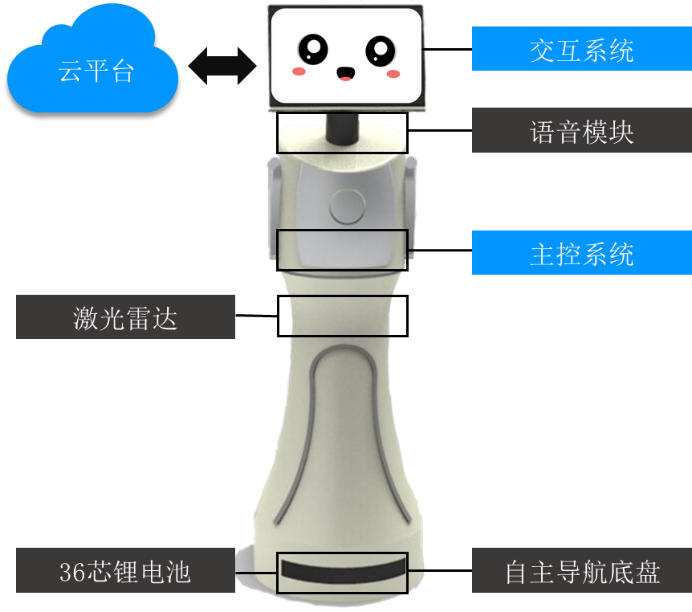
\includegraphics[width=0.5\textwidth]{example//overallstruct.png}
  \caption{智能医疗机器人整体结构}\label{overall_struct}
\end{figure}
主控系统通过协调控制语音、激光雷达、导航底盘等技术模块,实现机器人的拟人化功能输出;交互系统通过人机交互界面提供医疗服务,并实现机器人的可视化控制;云存储平台是机器人的数据管理中枢,主要负责动态数据的存储、管理与分析。智能医疗机器人各控制端的定位与运行机制如图\ref{flowchart}所示。\par
\begin{figure}[htbp]
  \centering
  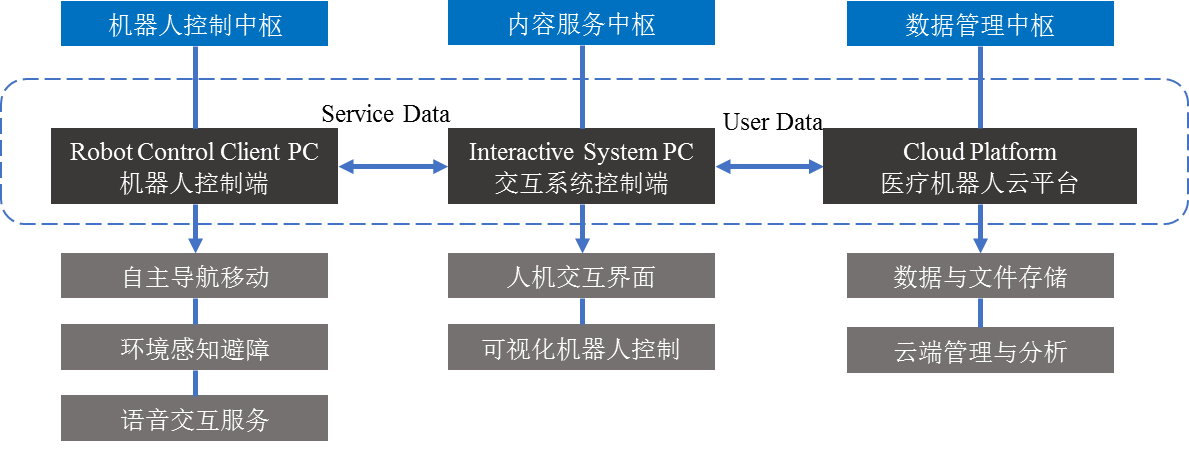
\includegraphics[width=0.8\textwidth]{example//flowchart.png}
  \caption{各控制端的定位与运行机制}\label{flowchart}
\end{figure}
智能医疗机器人软件系统架构如图2-3所示。基于ROS机器人操作系统开发的机器人控制端,可统一处理各功能硬件的数据,并将其转化为机器人行为输出。采用Android平台开发的交互系统控制端,首先可保持与云存储平台之间的实时数据通信,其次保持与主控制端之间的数据通信,从而控制机器人进行正确的行为输出。

\section{交互系统设计及实现}
\subsection{需求分析与架构设计}
根据应用场景和设计目标,智能医疗机器人的需求归纳如下:在功能方面,划分为体征监测、远程随访、智能医嘱、康复进度反馈、机器人控制、用户管理等模块;在数据管理方面,需保证所有云端数据的本地实时更新;在界面设计方面,交互系统界面架构要合理划分,在视觉体验上要具有时代感。根据需求,选择了Android作为交互系统开发平台。进行内容服务模块页面的重组划分,如图\ref{module}所示。
\begin{figure}[htbp]
  \centering
  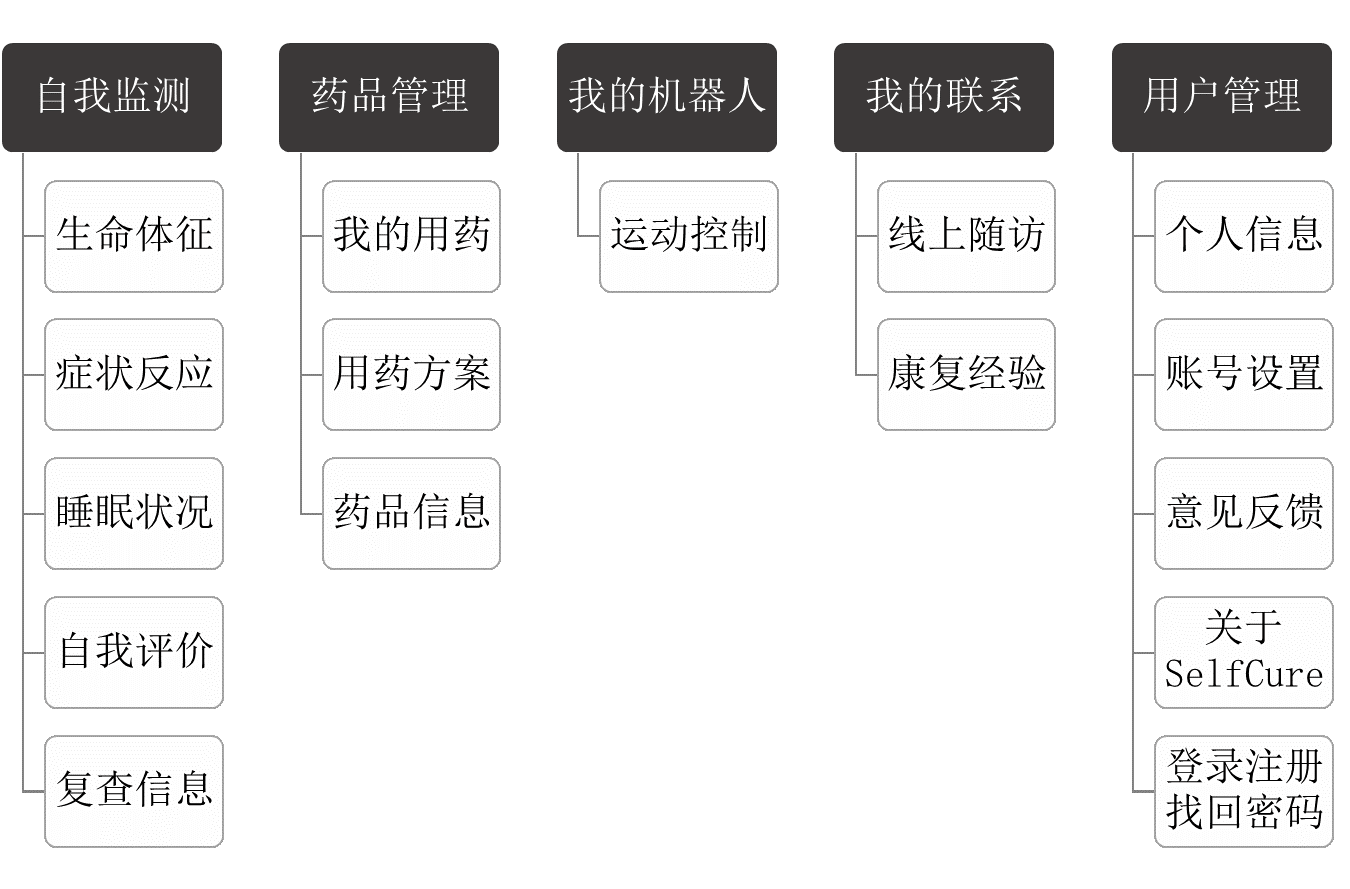
\includegraphics[width=0.5\textwidth]{example//module.png}
  \caption{内容服务模块划分}\label{module}
\end{figure}
交互系统的项目架构部署如图3-2所示。除了编译所需的配置与相关代码编写,主要关注前端静态界面res和后端功能实现java两部分内容。\par
\subsection{交互系统UI设计}
通过人机学研究,最终选择了\# 0195ff道奇蓝、\# 404040深灰、\# f0f0f6淡灰、\# fffafa雪白作为主题色,并设计了机器人产品LOGO与部分素材,如图3-3所示。\par
由于Android官方库有限,因此编写制作了滑动选择器、底部弹出式选择框、确认与取消提示框等UI控件。部分控件如图3-4所示。

\subsection{界面设计与功能实现}
\subsubsection{主页面模块}
主页面与机器人形象动态页面如图3-5所示。主页面采用了底栏和顶栏的双级目录结构,旨在使用户可以通过少于两步操作到达任何一个功能模块。通过顶栏右方的人形按键可以跳转至用户管理页面。为了使交互系统机器人化,实现操作静止20秒后会自动跳转机器人卡通形象,点击屏幕可以跳转回主页面。
\subsubsection{症状反应模块}
症状反应信息是医生对于患者康复情况判断的重要依据,该模块以选择题问卷的形式呈现,配合机器人周期性的智能提醒,患者可以方便且无遗漏地反馈症状情况;医生可实时查看患者症状反应信息统计,及时修改治疗方案,相关界面如图3-6所示。
\subsubsection{生命体征模块}
传统的体征数据反馈方式往往是通过医生向患者的问询,这种反馈模式容易造成信息有误或丢失。该模块旨在帮助医生对患者形成有效的健康体征数据的远程监控。该模块界面如图3-8所示。
\subsubsection{常用工具封装}
“封装性”是JAVA语言的重要特点。本节实现了SharedPreference存储工具、缓存清理工具、文本格式判断工具的封装。缓存清理工具封装流程如表\ref{fuhao}所示。
\begin{table}[htbp]
  \centering
\begin{tabular}{|c|c|}
  \hline
  \makecell{符号}&\makecell{说明}\\ %makecell用于生成表头
  \hline
  $a_t$ & 参数在t时刻的值 \\
  \cline{1-2}
  $\rho$ & 相关系数 \\
  \cline{1-2}
  $\boldsymbol{\omega}$ & 超平面方向向量 \\
  \hline
\end{tabular}
  \caption{符号说明}\label{fuhao}
\end{table}

\section{交互系统与主控系统信息通讯实现}
“封装性”是JAVA语言的重要特点。本节实现了SharedPreference存储工具、缓存清理工具、文本格式判断工具的封装。缓存清理工具封装流程如表\ref{haha}所示。
\begin{table}[htbp]
  \centering
\begin{tabular}{|c|c|}
  \hline
  \makecell{符号}&\makecell{说明}\\ %makecell用于生成表头
  \hline
  $a_t$ & 参数在t时刻的值 \\
  \cline{1-2}
  $\rho$ & 相关系数 \\
  \cline{1-2}
  $\boldsymbol{\omega}$ & 超平面方向向量 \\
  \cline{1-2}
   $b$ & 超平面偏置量 \\
  \cline{1-2}
  \hline
\end{tabular}
  \caption{符号说明}\label{haha}
\end{table}
\end{document} 